

\tikzset{every picture/.style={line width=0.75pt}} %set default line width to 0.75pt        

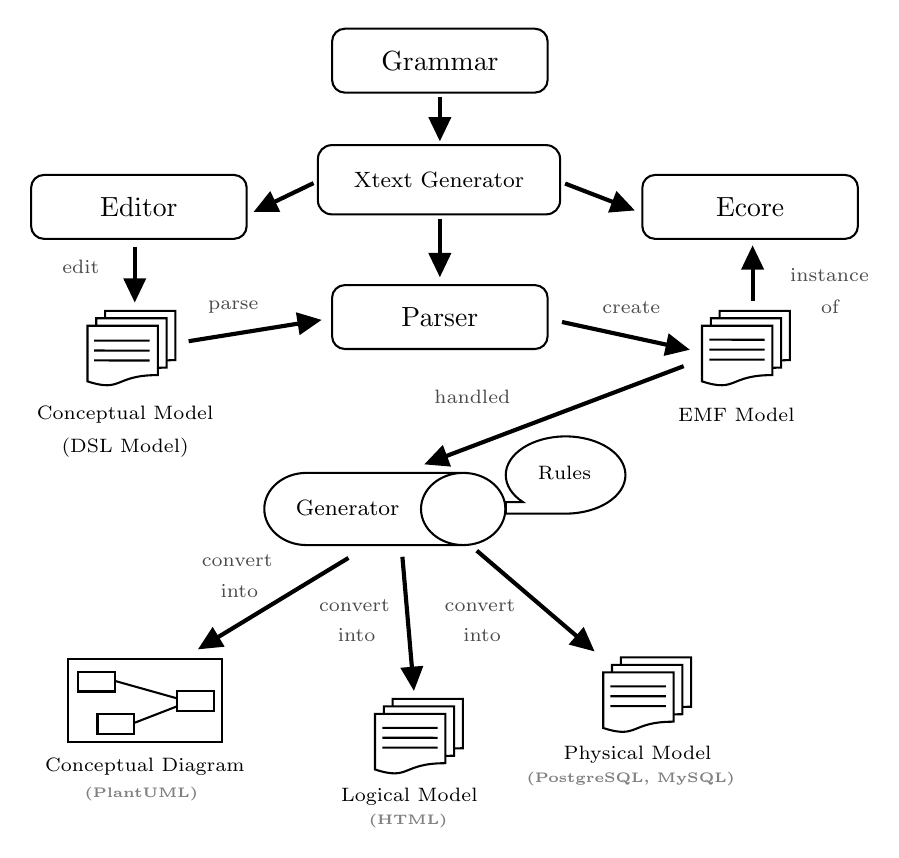
\begin{tikzpicture}[x=0.75pt,y=0.75pt,yscale=-1,xscale=1]
%uncomment if require: \path (0,465); %set diagram left start at 0, and has height of 465


%Rounded Rect [id:dp8080613887465731] 
\draw  [fill={rgb, 255:red, 255; green, 255; blue, 255 }  ,fill opacity=1 ] (268.24,22.37) .. controls (268.24,18.97) and (271,16.21) .. (274.4,16.21) -- (365.96,16.21) .. controls (369.36,16.21) and (372.11,18.97) .. (372.11,22.37) -- (372.11,40.84) .. controls (372.11,44.24) and (369.36,47) .. (365.96,47) -- (274.4,47) .. controls (271,47) and (268.24,44.24) .. (268.24,40.84) -- cycle ;
%Rounded Rect [id:dp23877247410758984] 
\draw  [fill={rgb, 255:red, 255; green, 255; blue, 255 }  ,fill opacity=1 ][line width=0.75]  (123.24,92.82) .. controls (123.24,89.42) and (126,86.66) .. (129.4,86.66) -- (220.95,86.66) .. controls (224.36,86.66) and (227.11,89.42) .. (227.11,92.82) -- (227.11,111.3) .. controls (227.11,114.7) and (224.36,117.46) .. (220.95,117.46) -- (129.4,117.46) .. controls (126,117.46) and (123.24,114.7) .. (123.24,111.3) -- cycle ;
%Flowchart: Multidocument [id:dp49717070559395604] 
\draw  [fill={rgb, 255:red, 255; green, 255; blue, 255 }  ,fill opacity=1 ] (158.88,152.12) -- (192.75,152.12) -- (192.75,175.89) .. controls (171.58,175.89) and (175.82,184.46) .. (158.88,178.91) -- cycle ; \draw  [fill={rgb, 255:red, 255; green, 255; blue, 255 }  ,fill opacity=1 ] (154.64,155.72) -- (188.52,155.72) -- (188.52,179.49) .. controls (167.35,179.49) and (171.58,188.06) .. (154.64,182.52) -- cycle ; \draw  [fill={rgb, 255:red, 255; green, 255; blue, 255 }  ,fill opacity=1 ] (150.41,159.32) -- (184.28,159.32) -- (184.28,183.09) .. controls (163.11,183.09) and (167.35,191.66) .. (150.41,186.12) -- cycle ;
%Straight Lines [id:da5642847406466045] 
\draw [fill={rgb, 255:red, 255; green, 255; blue, 255 }  ,fill opacity=1 ]   (153.63,166.47) -- (180.34,166.5) ;
%Straight Lines [id:da9779186616916171] 
\draw [fill={rgb, 255:red, 255; green, 255; blue, 255 }  ,fill opacity=1 ]   (153.63,171.26) -- (180.34,171.28) ;
%Straight Lines [id:da8217185402464098] 
\draw [fill={rgb, 255:red, 255; green, 255; blue, 255 }  ,fill opacity=1 ]   (153.63,176.04) -- (180.34,176.06) ;


%Straight Lines [id:da27204357118531197] 
\draw [fill={rgb, 255:red, 255; green, 255; blue, 255 }  ,fill opacity=1 ][line width=1.5]    (173.18,121.3) -- (173.18,144.06) ;
\draw [shift={(173.18,148.06)}, rotate = 270] [fill={rgb, 255:red, 0; green, 0; blue, 0 }  ][line width=0.08]  [draw opacity=0] (11.61,-5.58) -- (0,0) -- (11.61,5.58) -- cycle    ;
%Rounded Rect [id:dp014713549076222021] 
\draw  [fill={rgb, 255:red, 255; green, 255; blue, 255 }  ,fill opacity=1 ] (261.43,78.98) .. controls (261.43,75.3) and (264.41,72.31) .. (268.09,72.31) -- (371.45,72.31) .. controls (375.13,72.31) and (378.11,75.3) .. (378.11,78.98) -- (378.11,98.98) .. controls (378.11,102.66) and (375.13,105.65) .. (371.45,105.65) -- (268.09,105.65) .. controls (264.41,105.65) and (261.43,102.66) .. (261.43,98.98) -- cycle ;
%Rounded Rect [id:dp8159423215616721] 
\draw  [fill={rgb, 255:red, 255; green, 255; blue, 255 }  ,fill opacity=1 ] (417.72,92.82) .. controls (417.72,89.42) and (420.48,86.66) .. (423.88,86.66) -- (515.44,86.66) .. controls (518.84,86.66) and (521.59,89.42) .. (521.59,92.82) -- (521.59,111.3) .. controls (521.59,114.7) and (518.84,117.46) .. (515.44,117.46) -- (423.88,117.46) .. controls (420.48,117.46) and (417.72,114.7) .. (417.72,111.3) -- cycle ;
%Flowchart: Multidocument [id:dp814245162277164] 
\draw  [fill={rgb, 255:red, 255; green, 255; blue, 255 }  ,fill opacity=1 ] (454.96,152.12) -- (488.83,152.12) -- (488.83,175.89) .. controls (467.66,175.89) and (471.89,184.46) .. (454.96,178.91) -- cycle ; \draw  [fill={rgb, 255:red, 255; green, 255; blue, 255 }  ,fill opacity=1 ] (450.72,155.72) -- (484.6,155.72) -- (484.6,179.49) .. controls (463.43,179.49) and (467.66,188.06) .. (450.72,182.52) -- cycle ; \draw  [fill={rgb, 255:red, 255; green, 255; blue, 255 }  ,fill opacity=1 ] (446.49,159.32) -- (480.36,159.32) -- (480.36,183.09) .. controls (459.19,183.09) and (463.43,191.66) .. (446.49,186.12) -- cycle ;
%Straight Lines [id:da659202853659377] 
\draw [fill={rgb, 255:red, 255; green, 255; blue, 255 }  ,fill opacity=1 ]   (449.97,166.04) -- (476.69,166.06) ;
%Straight Lines [id:da8271632436642871] 
\draw [fill={rgb, 255:red, 255; green, 255; blue, 255 }  ,fill opacity=1 ]   (449.97,170.82) -- (476.69,170.85) ;
%Straight Lines [id:da22701123408508272] 
\draw [fill={rgb, 255:red, 255; green, 255; blue, 255 }  ,fill opacity=1 ]   (449.97,175.61) -- (476.69,175.63) ;


%Straight Lines [id:da6612735011438882] 
\draw [fill={rgb, 255:red, 255; green, 255; blue, 255 }  ,fill opacity=1 ][line width=1.5]    (470.86,124.65) -- (470.86,147.4) ;
\draw [shift={(470.86,120.65)}, rotate = 90] [fill={rgb, 255:red, 0; green, 0; blue, 0 }  ][line width=0.08]  [draw opacity=0] (11.61,-5.58) -- (0,0) -- (11.61,5.58) -- cycle    ;
%Rounded Rect [id:dp9641259565957541] 
\draw  [fill={rgb, 255:red, 255; green, 255; blue, 255 }  ,fill opacity=1 ] (268.24,145.89) .. controls (268.24,142.48) and (271,139.73) .. (274.4,139.73) -- (365.96,139.73) .. controls (369.36,139.73) and (372.11,142.48) .. (372.11,145.89) -- (372.11,164.36) .. controls (372.11,167.76) and (369.36,170.52) .. (365.96,170.52) -- (274.4,170.52) .. controls (271,170.52) and (268.24,167.76) .. (268.24,164.36) -- cycle ;
%Straight Lines [id:da4555835119587406] 
\draw [fill={rgb, 255:red, 255; green, 255; blue, 255 }  ,fill opacity=1 ][line width=1.5]    (320.18,48.89) -- (320.18,66.42) ;
\draw [shift={(320.18,70.42)}, rotate = 270] [fill={rgb, 255:red, 0; green, 0; blue, 0 }  ][line width=0.08]  [draw opacity=0] (11.61,-5.58) -- (0,0) -- (11.61,5.58) -- cycle    ;
%Straight Lines [id:da2586670416419199] 
\draw [fill={rgb, 255:red, 255; green, 255; blue, 255 }  ,fill opacity=1 ][line width=1.5]    (320.18,107.78) -- (320.18,131.88) ;
\draw [shift={(320.18,135.88)}, rotate = 270] [fill={rgb, 255:red, 0; green, 0; blue, 0 }  ][line width=0.08]  [draw opacity=0] (11.61,-5.58) -- (0,0) -- (11.61,5.58) -- cycle    ;
%Straight Lines [id:da2552674310073062] 
\draw [fill={rgb, 255:red, 255; green, 255; blue, 255 }  ,fill opacity=1 ][line width=1.5]    (259.32,90.59) -- (234.04,102.77) ;
\draw [shift={(230.43,104.51)}, rotate = 334.28] [fill={rgb, 255:red, 0; green, 0; blue, 0 }  ][line width=0.08]  [draw opacity=0] (11.61,-5.58) -- (0,0) -- (11.61,5.58) -- cycle    ;
%Straight Lines [id:da29550662771480396] 
\draw [fill={rgb, 255:red, 255; green, 255; blue, 255 }  ,fill opacity=1 ][line width=1.5]    (410.34,102.31) -- (380.52,90.81) ;
\draw [shift={(414.07,103.76)}, rotate = 201.11] [fill={rgb, 255:red, 0; green, 0; blue, 0 }  ][line width=0.08]  [draw opacity=0] (11.61,-5.58) -- (0,0) -- (11.61,5.58) -- cycle    ;
%Straight Lines [id:da3280771928101003] 
\draw [fill={rgb, 255:red, 255; green, 255; blue, 255 }  ,fill opacity=1 ][line width=1.5]    (199.15,166.77) -- (259.22,157.13) ;
\draw [shift={(263.17,156.5)}, rotate = 530.89] [fill={rgb, 255:red, 0; green, 0; blue, 0 }  ][line width=0.08]  [draw opacity=0] (11.61,-5.58) -- (0,0) -- (11.61,5.58) -- cycle    ;
%Straight Lines [id:da9478402467031726] 
\draw [fill={rgb, 255:red, 255; green, 255; blue, 255 }  ,fill opacity=1 ][line width=1.5]    (379.03,157.51) -- (436.63,170.02) ;
\draw [shift={(440.54,170.87)}, rotate = 192.26] [fill={rgb, 255:red, 0; green, 0; blue, 0 }  ][line width=0.08]  [draw opacity=0] (11.61,-5.58) -- (0,0) -- (11.61,5.58) -- cycle    ;
%Flowchart: Direct Access Storage [id:dp7657317583515377] 
\draw  [fill={rgb, 255:red, 255; green, 255; blue, 255 }  ,fill opacity=1 ] (331.43,264.99) -- (255.92,264.99) .. controls (244.69,264.99) and (235.59,257.2) .. (235.59,247.6) .. controls (235.59,238) and (244.69,230.21) .. (255.92,230.21) -- (331.43,230.21)(351.75,247.6) .. controls (351.75,257.2) and (342.65,264.99) .. (331.43,264.99) .. controls (320.2,264.99) and (311.1,257.2) .. (311.1,247.6) .. controls (311.1,238) and (320.2,230.21) .. (331.43,230.21) .. controls (342.65,230.21) and (351.75,238) .. (351.75,247.6) ;
%Straight Lines [id:da100480350897858] 
\draw [fill={rgb, 255:red, 255; green, 255; blue, 255 }  ,fill opacity=1 ][line width=1.5]    (437.65,178.79) -- (316.46,224.67) ;
\draw [shift={(312.72,226.08)}, rotate = 339.27] [fill={rgb, 255:red, 0; green, 0; blue, 0 }  ][line width=0.08]  [draw opacity=0] (11.61,-5.58) -- (0,0) -- (11.61,5.58) -- cycle    ;
%Flowchart: Multidocument [id:dp5253239734010293] 
\draw  [fill={rgb, 255:red, 255; green, 255; blue, 255 }  ,fill opacity=1 ] (297.41,339.12) -- (331.29,339.12) -- (331.29,362.88) .. controls (310.11,362.88) and (314.35,371.45) .. (297.41,365.91) -- cycle ; \draw  [fill={rgb, 255:red, 255; green, 255; blue, 255 }  ,fill opacity=1 ] (293.18,342.72) -- (327.05,342.72) -- (327.05,366.48) .. controls (305.88,366.48) and (310.11,375.05) .. (293.18,369.51) -- cycle ; \draw  [fill={rgb, 255:red, 255; green, 255; blue, 255 }  ,fill opacity=1 ] (288.94,346.32) -- (322.82,346.32) -- (322.82,370.08) .. controls (301.65,370.08) and (305.88,378.66) .. (288.94,373.11) -- cycle ;
%Straight Lines [id:da29635223798470123] 
\draw [fill={rgb, 255:red, 255; green, 255; blue, 255 }  ,fill opacity=1 ]   (292.43,353.03) -- (319.14,353.05) ;
%Straight Lines [id:da45709195099870326] 
\draw [fill={rgb, 255:red, 255; green, 255; blue, 255 }  ,fill opacity=1 ]   (292.43,357.82) -- (319.14,357.84) ;
%Straight Lines [id:da9397926099052756] 
\draw [fill={rgb, 255:red, 255; green, 255; blue, 255 }  ,fill opacity=1 ]   (292.43,362.6) -- (319.14,362.62) ;




%Straight Lines [id:da10826901476686546] 
\draw [fill={rgb, 255:red, 255; green, 255; blue, 255 }  ,fill opacity=1 ][line width=1.5]    (302.13,270.64) -- (307.34,331.21) ;
\draw [shift={(307.68,335.2)}, rotate = 265.08] [fill={rgb, 255:red, 0; green, 0; blue, 0 }  ][line width=0.08]  [draw opacity=0] (11.61,-5.58) -- (0,0) -- (11.61,5.58) -- cycle    ;
%Flowchart: Sequential Access Storage [id:dp3007368871754543] 
\draw  [fill={rgb, 255:red, 255; green, 255; blue, 255 }  ,fill opacity=1 ] (409.6,231.24) .. controls (409.6,220.96) and (396.69,212.63) .. (380.76,212.63) .. controls (364.84,212.63) and (351.93,220.96) .. (351.93,231.24) .. controls (351.93,236.31) and (355.07,240.9) .. (360.17,244.26) -- (351.93,244.26) -- (351.93,249.84) -- (380.76,249.84) .. controls (396.69,249.84) and (409.6,241.51) .. (409.6,231.24) -- cycle ;
%Shape: Rectangle [id:dp03278310257286665] 
\draw   (141.03,319.87) -- (215.03,319.87) -- (215.03,359.87) -- (141.03,359.87) -- cycle ;
%Shape: Rectangle [id:dp9445861445312367] 
\draw   (145.83,326.14) -- (163.55,326.14) -- (163.55,335.52) -- (145.83,335.52) -- cycle ;
%Shape: Rectangle [id:dp035309426832852875] 
\draw   (193.63,335.34) -- (211.34,335.34) -- (211.34,344.72) -- (193.63,344.72) -- cycle ;
%Shape: Rectangle [id:dp0682098761538128] 
\draw   (155.23,346.54) -- (172.94,346.54) -- (172.94,355.92) -- (155.23,355.92) -- cycle ;
%Straight Lines [id:da09626722375251995] 
\draw    (172.65,350.78) -- (193.32,342.78) ;
%Straight Lines [id:da41470258123307224] 
\draw    (163.65,330.44) -- (193.32,338.78) ;


%Straight Lines [id:da24414024149042923] 
\draw [fill={rgb, 255:red, 255; green, 255; blue, 255 }  ,fill opacity=1 ][line width=1.5]    (276.13,271.19) -- (207.1,313.12) ;
\draw [shift={(203.68,315.2)}, rotate = 328.72] [fill={rgb, 255:red, 0; green, 0; blue, 0 }  ][line width=0.08]  [draw opacity=0] (11.61,-5.58) -- (0,0) -- (11.61,5.58) -- cycle    ;
%Flowchart: Multidocument [id:dp9410827405643849] 
\draw  [fill={rgb, 255:red, 255; green, 255; blue, 255 }  ,fill opacity=1 ] (407.36,319.12) -- (441.24,319.12) -- (441.24,342.88) .. controls (420.07,342.88) and (424.3,351.45) .. (407.36,345.91) -- cycle ; \draw  [fill={rgb, 255:red, 255; green, 255; blue, 255 }  ,fill opacity=1 ] (403.13,322.72) -- (437.01,322.72) -- (437.01,346.48) .. controls (415.83,346.48) and (420.07,355.05) .. (403.13,349.51) -- cycle ; \draw  [fill={rgb, 255:red, 255; green, 255; blue, 255 }  ,fill opacity=1 ] (398.89,326.32) -- (432.77,326.32) -- (432.77,350.08) .. controls (411.6,350.08) and (415.83,358.66) .. (398.89,353.11) -- cycle ;
%Straight Lines [id:da31801059922861796] 
\draw [fill={rgb, 255:red, 255; green, 255; blue, 255 }  ,fill opacity=1 ]   (402.38,333.03) -- (429.1,333.05) ;
%Straight Lines [id:da19940799584772861] 
\draw [fill={rgb, 255:red, 255; green, 255; blue, 255 }  ,fill opacity=1 ]   (402.38,337.82) -- (429.1,337.84) ;
%Straight Lines [id:da720164043002747] 
\draw [fill={rgb, 255:red, 255; green, 255; blue, 255 }  ,fill opacity=1 ]   (402.38,342.6) -- (429.1,342.62) ;




%Straight Lines [id:da4341747356667731] 
\draw [fill={rgb, 255:red, 255; green, 255; blue, 255 }  ,fill opacity=1 ][line width=1.5]    (337.96,267.69) -- (391.64,313.6) ;
\draw [shift={(394.68,316.2)}, rotate = 220.53] [fill={rgb, 255:red, 0; green, 0; blue, 0 }  ][line width=0.08]  [draw opacity=0] (11.61,-5.58) -- (0,0) -- (11.61,5.58) -- cycle    ;



% Text Node
\draw (175.18,102.06) node   [align=left] {Editor};
% Text Node
\draw (469.66,102.06) node   [align=left] {Ecore};
% Text Node
\draw (320.18,155.12) node   [align=left] {Parser};
% Text Node
\draw (320.18,31.6) node  [font=\normalsize] [align=left] {Grammar};
% Text Node
\draw (168.54,201.99) node   [align=left] {{\scriptsize Conceptual Model}};
% Text Node
\draw (463.03,201.99) node   [align=left] {{\scriptsize EMF Model}};
% Text Node
\draw (275.76,247.14) node  [font=\footnotesize] [align=left] {\begin{minipage}[lt]{39.43pt}\setlength\topsep{0pt}
\begin{center}
Generator
\end{center}

\end{minipage}};
% Text Node
\draw (380.24,230.37) node  [font=\scriptsize] [align=left] {\begin{minipage}[lt]{20.96pt}\setlength\topsep{0pt}
\begin{center}
Rules
\end{center}

\end{minipage}};
% Text Node
\draw (136.8,126.16) node [anchor=north west][inner sep=0.75pt]  [font=\scriptsize,color={rgb, 255:red, 74; green, 74; blue, 74 }  ,opacity=1 ] [align=left] {edit};
% Text Node
\draw (207,146.18) node [anchor=north west][inner sep=0.75pt]  [font=\scriptsize,color={rgb, 255:red, 74; green, 74; blue, 74 }  ,opacity=1 ] [align=left] {parse};
% Text Node
\draw (397,146.18) node [anchor=north west][inner sep=0.75pt]  [font=\scriptsize,color={rgb, 255:red, 74; green, 74; blue, 74 }  ,opacity=1 ] [align=left] {create};
% Text Node
\draw (487.4,130.21) node [anchor=north west][inner sep=0.75pt]  [font=\scriptsize,color={rgb, 255:red, 74; green, 74; blue, 74 }  ,opacity=1 ] [align=left] {instance};
% Text Node
\draw (316,188.69) node [anchor=north west][inner sep=0.75pt]  [font=\scriptsize,color={rgb, 255:red, 74; green, 74; blue, 74 }  ,opacity=1 ] [align=left] {handled};
% Text Node
\draw (502.4,145.21) node [anchor=north west][inner sep=0.75pt]  [font=\scriptsize,color={rgb, 255:red, 74; green, 74; blue, 74 }  ,opacity=1 ] [align=left] {of};
% Text Node
\draw (319.77,88.98) node  [font=\footnotesize] [align=left] {Xtext Generator};
% Text Node
\draw (168.54,217.99) node   [align=left] {{\scriptsize (DSL Model)}};
% Text Node
\draw (204,268.3) node [anchor=north west][inner sep=0.75pt]  [font=\scriptsize,color={rgb, 255:red, 74; green, 74; blue, 74 }  ,opacity=1 ] [align=left] {convert};
% Text Node
\draw (213,282.3) node [anchor=north west][inner sep=0.75pt]  [font=\scriptsize,color={rgb, 255:red, 74; green, 74; blue, 74 }  ,opacity=1 ] [align=left] {into};
% Text Node
\draw (305.48,385.98) node   [align=left] {{\scriptsize Logical Model}};
% Text Node
\draw (415.43,365.98) node   [align=left] {{\scriptsize Physical Model}};
% Text Node
\draw (284.48,392.91) node [anchor=north west][inner sep=0.75pt]   [align=left] {{\tiny \textcolor[rgb]{0.5,0.5,0.5}{\textbf{(HTML)}}}};
% Text Node
\draw (360.43,372.91) node [anchor=north west][inner sep=0.75pt]   [align=left] {{\tiny \textcolor[rgb]{0.5,0.5,0.5}{\textbf{(PostgreSQL, MySQL)}}}};
% Text Node
\draw (147.53,380.15) node [anchor=north west][inner sep=0.75pt]   [align=left] {{\tiny \textcolor[rgb]{0.5,0.5,0.5}{\textbf{(PlantUML)}}}};
% Text Node
\draw (178.03,371.89) node   [align=left] {{\scriptsize Conceptual Diagram}};
% Text Node
\draw (269.5,303.8) node [anchor=north west][inner sep=0.75pt]  [font=\scriptsize,color={rgb, 255:red, 74; green, 74; blue, 74 }  ,opacity=1 ] [align=left] {into};
% Text Node
\draw (260.5,289.8) node [anchor=north west][inner sep=0.75pt]  [font=\scriptsize,color={rgb, 255:red, 74; green, 74; blue, 74 }  ,opacity=1 ] [align=left] {convert};
% Text Node
\draw (330,303.8) node [anchor=north west][inner sep=0.75pt]  [font=\scriptsize,color={rgb, 255:red, 74; green, 74; blue, 74 }  ,opacity=1 ] [align=left] {into};
% Text Node
\draw (321,289.8) node [anchor=north west][inner sep=0.75pt]  [font=\scriptsize,color={rgb, 255:red, 74; green, 74; blue, 74 }  ,opacity=1 ] [align=left] {convert};


\end{tikzpicture}
